%! alt A regular 20-sided polygon in its circle, with centre O. A triangle joins three of its vertices. Two of them are 5 sides apart, and the arc between them, made of 5 sides, is highlighted: it makes a right angle, 90 degrees, at O. The third vertex lies on the long arc, and the angle of the triangle there is 45 degrees, half of 90 degrees.
%! after_paragraph 1
%! scale 3
% The shared preamble of every Cevian figure. pipeline/figures turns these colours into theme-aware paint,
% and refuses any other colour, so draw only with them:
%   figink (lines and labels), figaux (construction lines), figaccent (the object the argument turns on),
%   figtint and figaccenttint (light fills).
\documentclass[border=1.5pt]{standalone}
\usepackage{tkz-euclide}
\definecolor{figink}{RGB}{0,0,0}
\definecolor{figaux}{RGB}{85,85,85}
\definecolor{figaccent}{RGB}{192,57,43}
\definecolor{figtint}{RGB}{221,221,221}
\definecolor{figaccenttint}{RGB}{245,213,208}
% tkz-euclide's defaults draw circles, compasses and marks in 50% grey and fill points with a tint.
\makeatletter
\def\tkz@otherlinecolor{figink}
\def\tkz@euc@circlecolor{figink}
\def\tkz@euc@compasscolor{figink}
\def\tkz@euc@mkcolor{figink}
\def\tkz@mk@fill{figink}
\def\tkz@euc@pointfillcolor{figink}
\makeatother
\tkzSetUpLine[color=figink,line width=.7pt]
\tkzSetUpArc[color=figink,line width=.7pt]
\tkzSetUpCompass[color=figink,line width=.5pt]
\tkzSetUpPoint[color=figink,fill=figink,size=3.1pt]
\tikzset{
  every picture/.style={line cap=round,line join=round,color=figink},
  circle style/.append style={color=figink,line width=.7pt},
  aux/.style={color=figaux,line width=.45pt,dash pattern=on 2.6pt off 2pt},
  key/.style={color=figaccent,line width=1pt},
  mk/.style={color=figink,line width=.5pt},
  lbl/.style={color=figink,inner sep=2.2pt},
  len/.style={color=figink,inner sep=1.5pt,font=\small},
}

\begin{document}
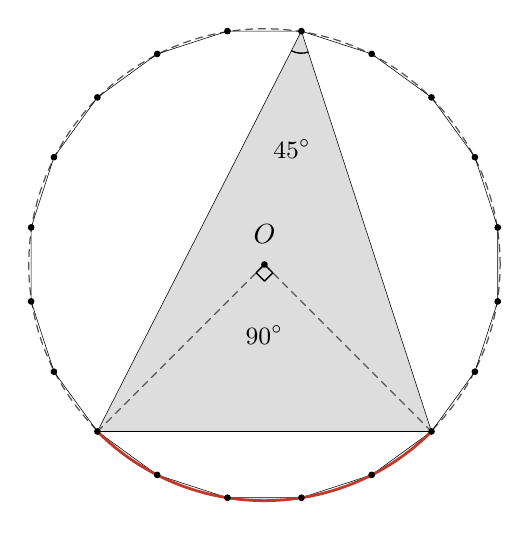
\begin{tikzpicture}
\tkzDefPoint(0.0,0.0){O} %! O = (0, 0)
\tkzDefPoint(-2.1213203,-2.1213203){V0} %! V0 = polar(O, 1, 225)
\tkzDefPoint(-1.3619715,-2.6730196){V1} %! V1 = polar(O, 1, 243)
\tkzDefPoint(-0.46930340,-2.9630650){V2} %! V2 = polar(O, 1, 261)
\tkzDefPoint(0.46930340,-2.9630650){V3} %! V3 = polar(O, 1, 279)
\tkzDefPoint(1.3619715,-2.6730196){V4} %! V4 = polar(O, 1, 297)
\tkzDefPoint(2.1213203,-2.1213203){V5} %! V5 = polar(O, 1, 315)
\tkzDefPoint(2.6730196,-1.3619715){V6} %! V6 = polar(O, 1, 333)
\tkzDefPoint(2.9630650,-0.46930340){V7} %! V7 = polar(O, 1, 351)
\tkzDefPoint(2.9630650,0.46930340){V8} %! V8 = polar(O, 1, 369)
\tkzDefPoint(2.6730196,1.3619715){V9} %! V9 = polar(O, 1, 387)
\tkzDefPoint(2.1213203,2.1213203){V10} %! V10 = polar(O, 1, 405)
\tkzDefPoint(1.3619715,2.6730196){V11} %! V11 = polar(O, 1, 423)
\tkzDefPoint(0.46930340,2.9630650){V12} %! V12 = polar(O, 1, 441)
\tkzDefPoint(-0.46930340,2.9630650){V13} %! V13 = polar(O, 1, 459)
\tkzDefPoint(-1.3619715,2.6730196){V14} %! V14 = polar(O, 1, 477)
\tkzDefPoint(-2.1213203,2.1213203){V15} %! V15 = polar(O, 1, 495)
\tkzDefPoint(-2.6730196,1.3619715){V16} %! V16 = polar(O, 1, 513)
\tkzDefPoint(-2.9630650,0.46930340){V17} %! V17 = polar(O, 1, 531)
\tkzDefPoint(-2.9630650,-0.46930340){V18} %! V18 = polar(O, 1, 549)
\tkzDefPoint(-2.6730196,-1.3619715){V19} %! V19 = polar(O, 1, 567)
\tkzDefPoint(0.35161475,1.4676890){L45} %! L45 = polar(V12, 0.5, 265.5)
\tkzDefPoint(-0.0000000000000000000000000000000000000000000000000058520255,-0.90000000){L90} %! L90 = polar(O, 0.3, 270)
\tkzDefPoint(0.00000000000000000000000000000000000000000000000000084529257,0.39000000){LO} %! LO = polar(O, 0.13, 90)
%! fact angle(V0, V12, V5) == 45
%! fact angle(V0, O, V5) == 90
%! fact dist(V0, V1) == dist(V11, V12)
%! example angle(V5, V0, V12) == 63
%! example angle(V0, V5, V12) == 72
\tkzFillPolygon[color=figtint](V0,V5,V12)
\tkzDrawCircle[aux](O,V0)
\tkzDrawPolygon(V0,V1,V2,V3,V4,V5,V6,V7,V8,V9,V10,V11,V12,V13,V14,V15,V16,V17,V18,V19)
\tkzDrawArc[key](O,V0)(V5)
\tkzDrawPolygon(V0,V5,V12)
\tkzDrawSegments[aux](O,V0 O,V5)
\tkzMarkAngle[size=.28,arc=l,mark=none,mk](V0,V12,V5)
\tkzMarkRightAngle[size=.15,mk](V0,O,V5)
\tkzDrawPoints(O,V0,V1,V2,V3,V4,V5,V6,V7,V8,V9,V10,V11,V12,V13,V14,V15,V16,V17,V18,V19)
\tkzLabelPoint[anchor=center,font=\small](L45){$45^\circ$}
\tkzLabelPoint[anchor=center,font=\small](L90){$90^\circ$}
\tkzLabelPoint[anchor=center,lbl](LO){$O$}
\end{tikzpicture}
\end{document}
